\newpage
\section{Results}


All figures shown in this section was produced using the CTCS scheme with
$\Delta x = \frac{1}{40} $ and $\Delta t = 0.10$.

\subsection{Periodic}

With periodic boundaries and a sinusoidal inital state (\Cref{fig:periodic_sine})
the phase speed is constant and all waves move westward. By following one wave
from east to west we can find the phase speed as $\frac{\Delta x}{\Delta t} =
\frac{0-1}{160} = -0.00625$.

\begin{figure}[htp]
  \centering
  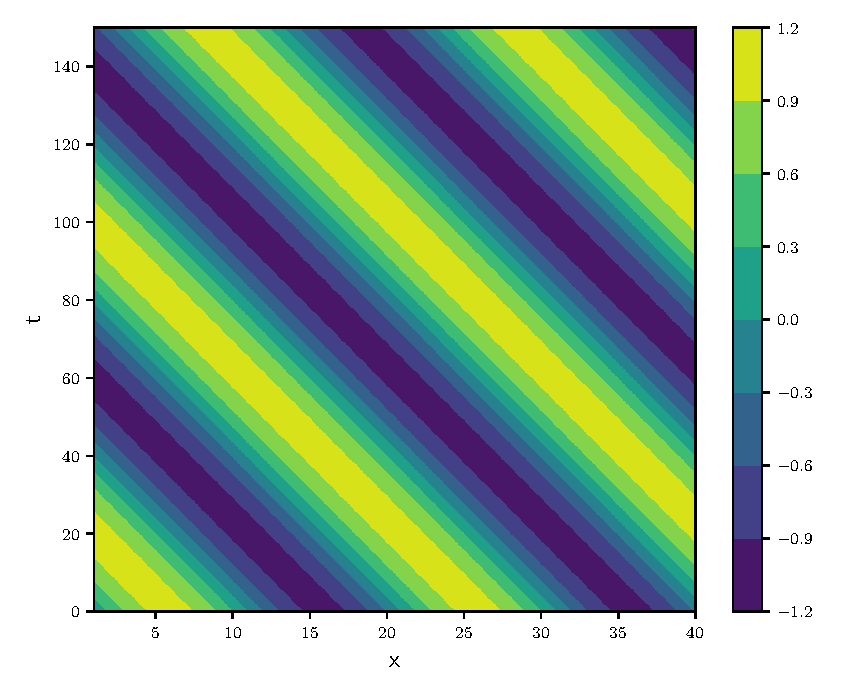
\includegraphics[width=\textwidth]{../figures/psi_periodic_centered_short.pdf}
  \caption{Hovmuller diagram for the periodic domain with a sinusoidal initial state. CTCS, $\Delta x = \frac{1}{40}$, $\Delta t = 0.10$. Waves propagate westward.}
  \label{fig:periodic_sine}
\end{figure}

With a Gaussian initial state (\cref{fig:periodic_gauss}) the Hovmöller diagram
is not as ordered. Due to the less order in the initial state the phase velocity
is not constant in time. This effect is most prominent for the cases where
$\sigma$ is small. For large $\sigma$ the phase velocity seems to be more
constant.


\begin{figure}[H]
  \centering
  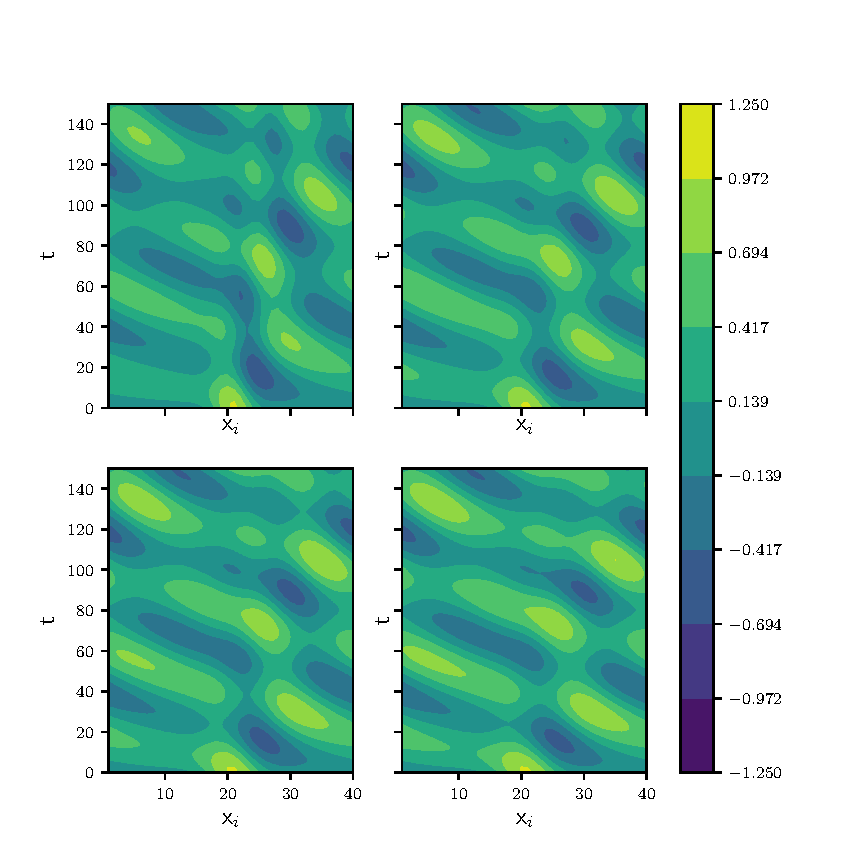
\includegraphics[width=\textwidth]{../figures/hovmuller_sigma.pdf}
  \caption{Hovmöller diagram for the periodic domain with a Gaussian initial
  state.From top left to bottom right: $\sigma = \brak{0.08, 0.10, 0.11, 0.12}$.
  CTCS, $\Delta x = \frac{1}{40}$, $\Delta t = 0.10$.
  }
  \label{fig:periodic_gauss}
\end{figure}



\subsection{Bounded}

With no flow at the boundaries and an initial sinusoidal \cref{fig:bounded_sine}
we can use the same method as for the periodic to find a phase speed of
$\frac{\Delta x}{\Delta t} = \frac{0 -1}{100 - 20} = -0.0125$.
The wave pattern fits well with the theoretical case. Since our initial state
has wave number 2 the sine term modulating the solution has one through and
one ridge, and is zero at both ends and the middle.


\begin{figure}[H]
  \centering
  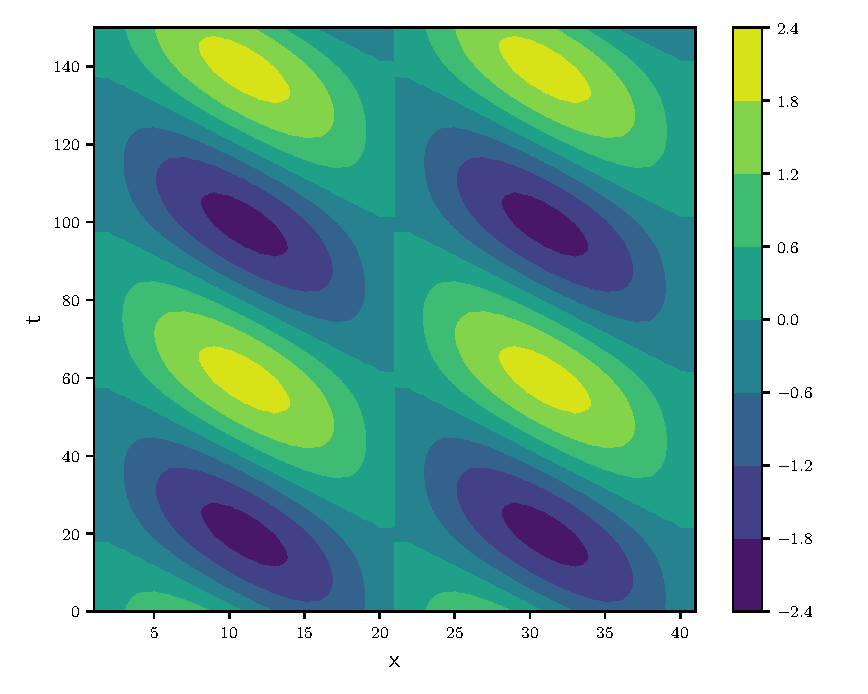
\includegraphics[width=\textwidth]{../figures/psi_bounded_centered_sine.pdf}
  \caption{Hovmuller diagram for the bounded domain with a sinusoidal initial
  state. CTCS, $\Delta x = \frac{1}{40}$, $\Delta t = 0.10$.}
  \label{fig:bounded_sine}
\end{figure}


\begin{figure}[H]
  \centering
  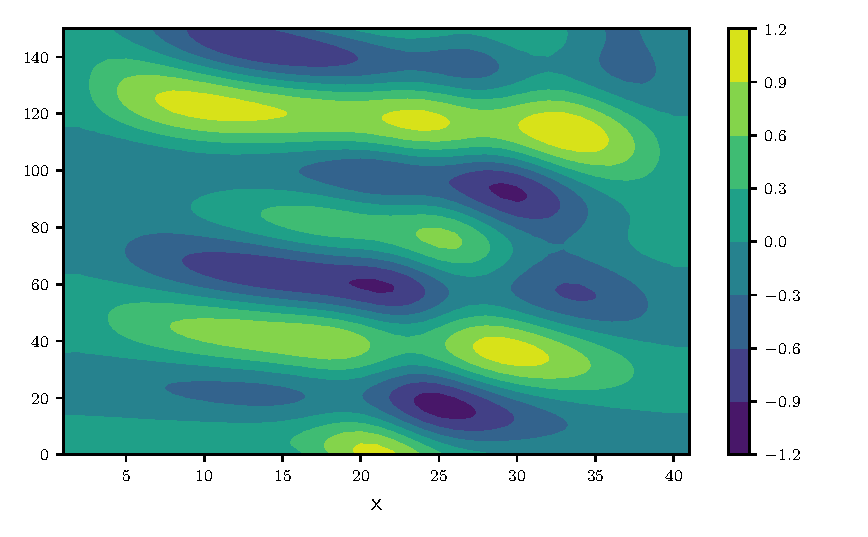
\includegraphics[width=\textwidth]{../figures/psi_bounded_centered_gauss.pdf}
  \caption{Hovmuller diagram for the bounded domain with a Gaussian initial state. CTCS, $\Delta x = \frac{1}{40}$, $\Delta t = 0.10$.}
  \label{fig:bounded_gauss}
\end{figure}


\subsection{2 dimensions}

In two dimensions we only looked at the sinusoidal initial state. With both
periodic (\cref{fig:2d_periodic}) and closed boundaries (\cref{fig:2d_bounded})
the waves seem to be travelling in very much the same way as in the one
dimensional case.

\begin{figure}[H]
  \centering
  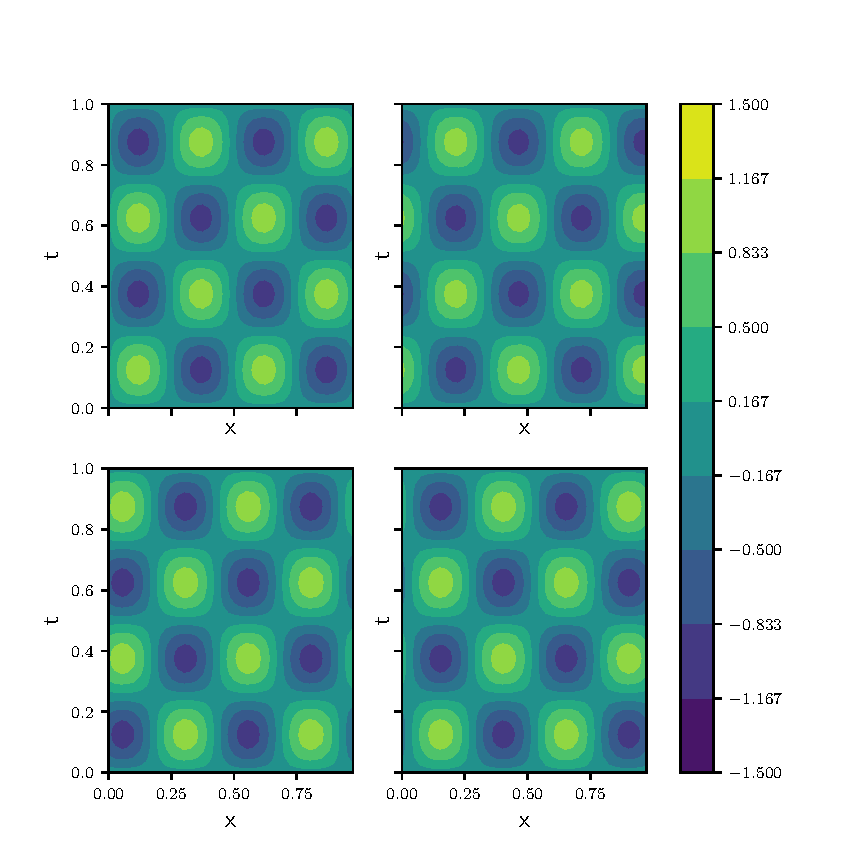
\includegraphics[width=\textwidth]{../figures/periodic_2d.pdf}
  \caption{Rossby wave travelling in a 2d periodic domain, plotted is the state of the wave at four different times. CTCS, $\Delta x = \Delta y = \frac{1}{40}$, $\Delta t = 0.10$.}
  \label{fig:2d_periodic}
\end{figure}



\begin{figure}[H]
  \centering
  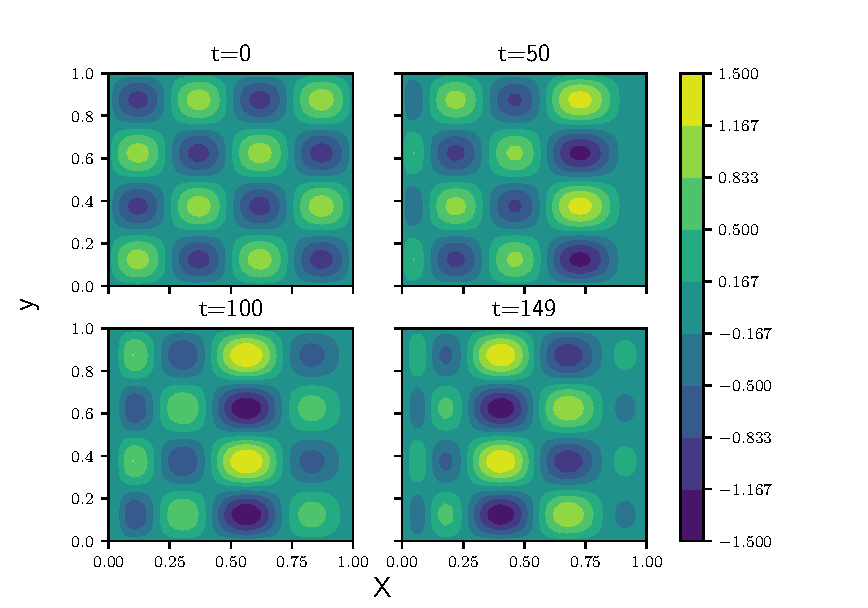
\includegraphics[width=\textwidth]{../figures/bounded_2d.pdf}
  \caption{Rossby wave travelling in a 2d basin, plotted is the state of the wave  at four different times. CTCS, $\Delta x = \Delta y = \frac{1}{40}$, $\Delta t = 0.10$.}
  \label{fig:2d_bounded}
\end{figure}
